\chapter{Fejlesztői dokumentáció} % Developer guide
\label{ch:impl}

\section{Feladat specifikáció}
Az webalkalmazás egy Single Page Applikáció (SPA), aminek a célja egy működő webáruház bemutatása Angular keretrendszerben. Az alkalmazás két főrészre osztható kliensoldali (front-end) és egy szerveroldali (back-end) részre. A kliensoldal feladata, hogy a felhasználó által látott UI/UX megjelenítést biztosítsa, amíg a szerveroldal felel a business logikáért, továbbá az adatok feldolgozásáért és autentikációjáért.

\begin{figure}[H]
	\centering
	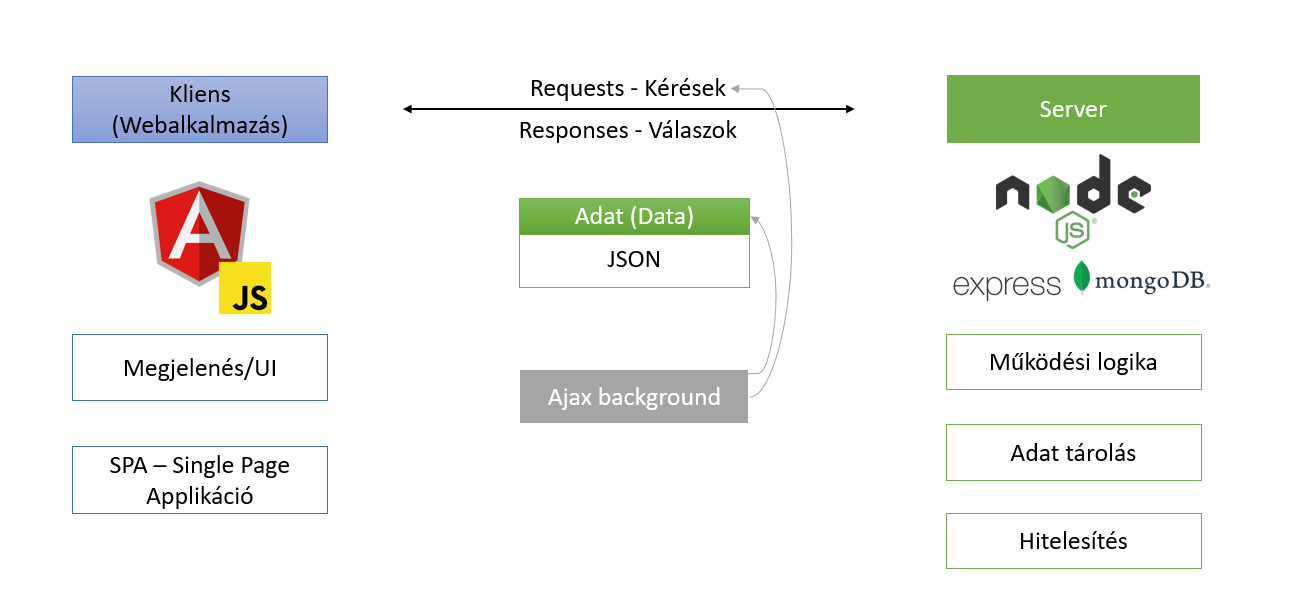
\includegraphics[width=1.0\textwidth,height=250px]{images/alkalmazas_bemutatasa.png}
	\caption{Az alkalmazás bemutatása}
	\label{fig.picture-1}
\end{figure}

A 3.1-es ábrán látható a két oldal kommunikációs kapcsolata. A front-end pontosabban mondva a kliensoldal Angular keretrendszerben TypeScript segítségével íródott. A front-end kommunikációja úgynevezett requestekkel kérésekkel (json típusú adattovábbítással) történik amire a szerver oldal responsokkal egyszóval válaszokkal felel. A back-end NodeJS szoftverrendszer alapú, ami Express segítségével íródott. Az adatok tárolásáért a MongoDB felel.

\section{Webalkalmazás radikális bemutatása}

\subsection{Kliensoldalon használt technológiák bemutatása}

\subsection{Kliensoldal működése}

\subsection{Szerveroldal használt technológiák bemutatása}

A következő fejezetben szeretném kifejteni a webáruház szerveroldali felépítését és működését. A 3.1-es ábrában felsorolt technológiákat részletesebben is bemutatni további ábrák segítségével.

\begin{figure}[H]
	\centering
	
\includegraphics[width=1.0\textwidth,height=220px]{images/nodejs_bemutatasa.png}
	\caption{NodeJS bemutatása}
	\label{fig.picture-3}
\end{figure}

A webáruház szerveroldala 14.15.4-es verziójú Node.js szoftverrendszert használ. A 3.2-es ábrán olvasható, hogy a Node.js skálázható internetes alkalmazások úgynevezett webszerverek készítésére alkalmas rendszer. A Node.js fogadja a kliensoldalról érkező kéréseket (requests) és válaszokat (responses) küld neki vissza.

\begin{figure}[H]
	\centering
	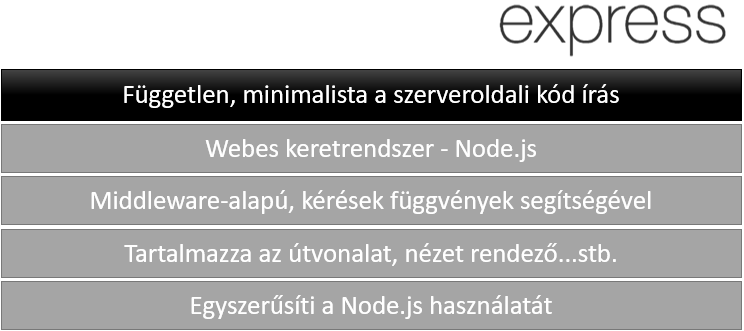
\includegraphics[width=1.0\textwidth,height=220px]{images/express_bemutatasa.png}
	\caption{Express bemutatása}
	\label{fig.picture-4}
\end{figure}

Express leírása

\begin{figure}[H]
	\centering
	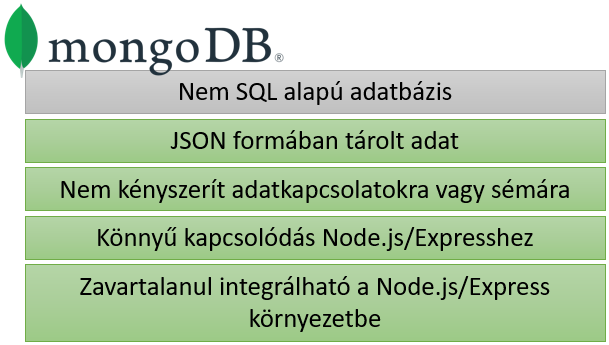
\includegraphics[width=1.0\textwidth,height=220px]{images/mongodb_bemutatasa.png}
	\caption{mongoDB bemutatása}
	\label{fig.picture-5}
\end{figure}

Adatbázis leírása:

\begin{figure}[H]
	\centering
	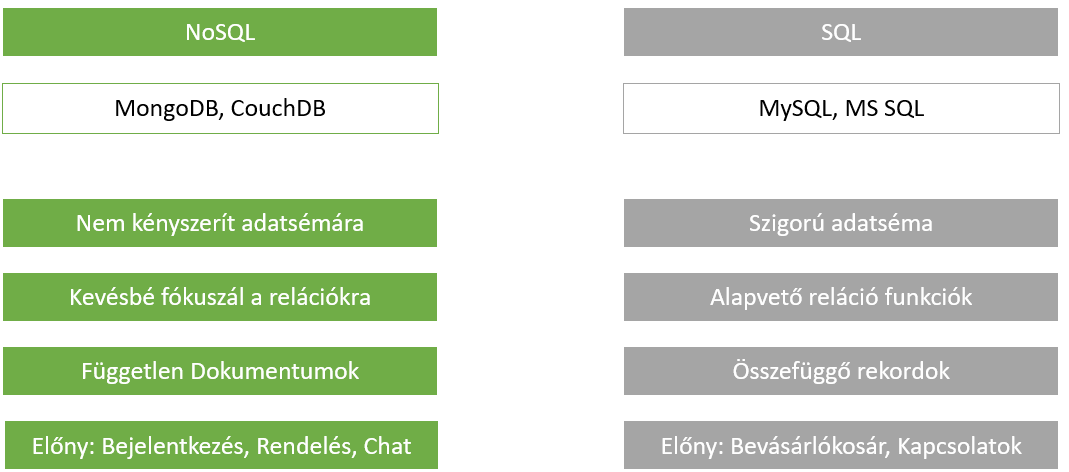
\includegraphics[width=1.0\textwidth,height=220px]{images/nosql_bemutatasa.png}
	\caption{NoSQL vs SQL adatbázisok összehasonlítása}
	\label{fig.picture-6}
\end{figure}

miért a mongodb előny hátrány?

\subsection{Szerveroldal működése}

restapi leírása:

\begin{figure}[H]
	\centering
	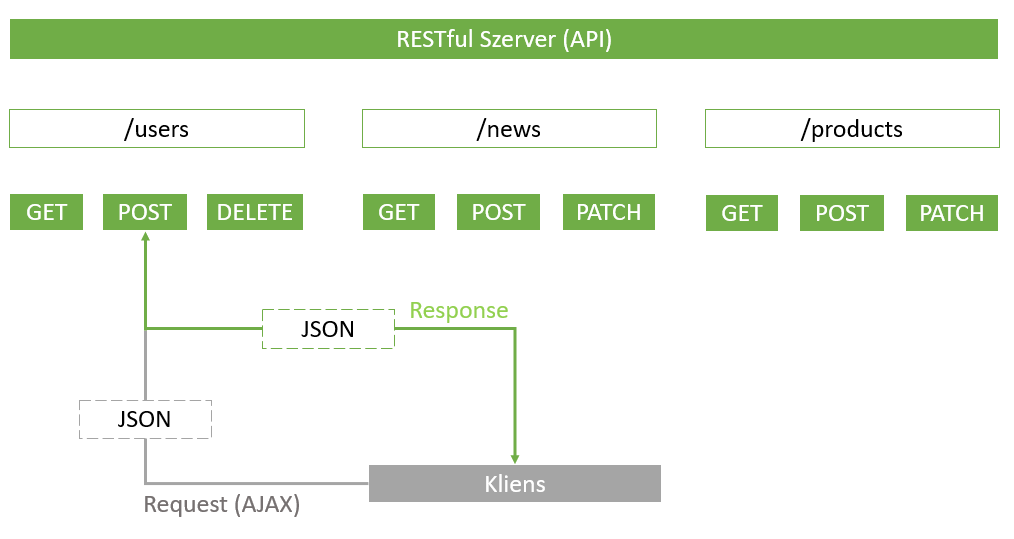
\includegraphics[width=1.0\textwidth,height=220px]{images/restapi_bemutatasa.png}
	\caption{Adatkezelés}
	\label{fig.picture-7}
\end{figure}

RESTAPI bemutatasa:

Alkalmazás admin felület védelem

\begin{figure}[H]
	\centering
	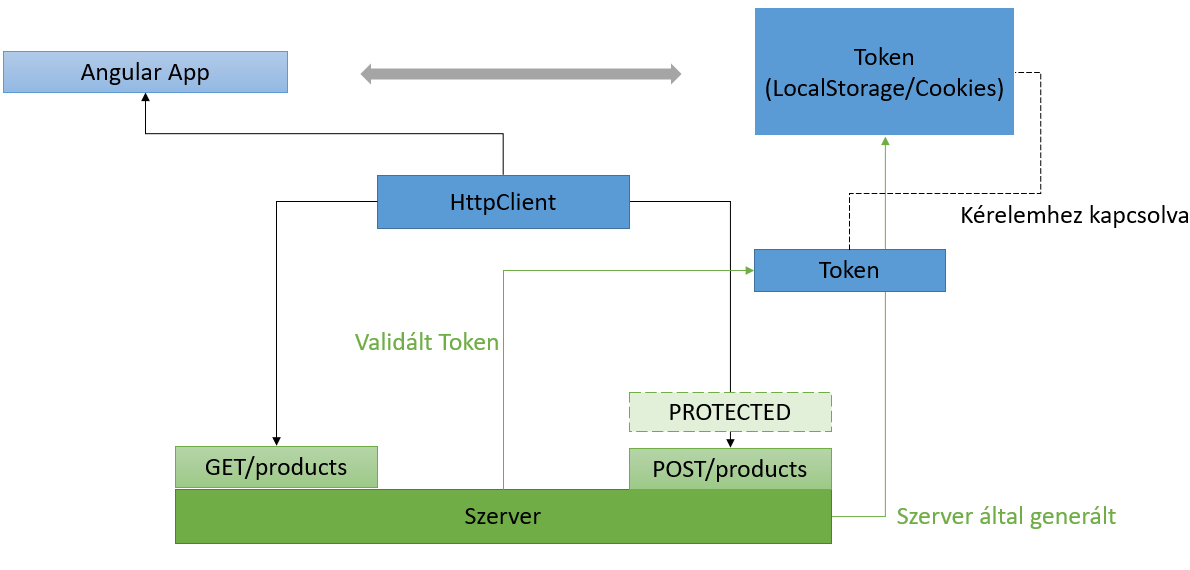
\includegraphics[width=1.0\textwidth,height=220px]{images/hitelesites_bemutatasa.png}
	\caption{Autentikáció}
	\label{fig.picture-8}
\end{figure}

Hitelesítés

\section{Tételek, definíciók, megjegyzések} % Theorem-like items

\begin{definition}
Mauris tristique sollicitudin ultrices. Etiam tristique quam sit amet metus dictum imperdiet. Nunc id lorem sed nisl pulvinar aliquet vitae quis arcu. Morbi iaculis eleifend porttitor.
\end{definition}

Maecenas rutrum eros sem, pharetra interdum nulla porttitor sit amet. In vitae viverra ante. Maecenas sit amet placerat orci, sed tincidunt velit. Vivamus mattis, enim vel suscipit elementum, quam odio venenatis elit, et mollis nulla nunc a risus. Praesent purus magna, tristique sed lacus sit amet, convallis malesuada magna. Phasellus faucibus varius purus, nec tristique enim porta vitae.

\begin{theorem}
Nulla finibus ante vel arcu tincidunt, ut consectetur ligula finibus. Mauris mollis lectus sed ipsum bibendum, ac ultrices erat dictum. Suspendisse faucibus euismod lacinia. Etiam vel odio ante.
\end{theorem}
\begin{proof}
Etiam pulvinar nibh quis massa auctor congue. Pellentesque quis odio vitae sapien molestie vestibulum sit amet et quam. Pellentesque vel dui eget enim hendrerit finibus at sit amet libero. Quisque sollicitudin ultrices enim, nec porta magna imperdiet vitae. Cras condimentum nunc dui.
\end{proof}

Donec dapibus sodales ante, at scelerisque nunc laoreet sit amet. Mauris porttitor tincidunt neque, vel ullamcorper neque pulvinar et. Integer eu lorem euismod, faucibus lectus sed, accumsan felis. 

\begin{remark}
Nunc ornare mi at augue vulputate, eu venenatis magna mollis. Nunc sed posuere dui, et varius nulla. Sed mollis nibh augue, eget scelerisque eros ornare nec. Praesent porta, metus eget eleifend consequat, eros ligula eleifend ex, a pellentesque mi est vitae urna. Vivamus turpis nunc, iaculis non leo eget, mattis vulputate tellus.
\end{remark}

Fusce in aliquet neque, in pretium sem. Donec tincidunt tellus id lectus pretium fringilla. Nunc faucibus, erat pretium tempus tempor, tortor mi fringilla neque, ac congue ex dui vitae mauris. Donec pretium et quam a cursus.

\begin{note}
Aliquam vehicula luctus mi a pretium. Nulla quam neque, maximus nec velit in, aliquam mollis tortor. Aliquam erat volutpat. Curabitur vitae laoreet turpis. Integer id diam ligula.
\end{note}

Ut sollicitudin tempus urna et mollis. Aliquam et aliquam turpis, sed fermentum mauris. Nulla eget ex diam. Donec eget tellus pharetra, semper neque eget, rutrum diam.

\subsection{Egyenletek, matematika} % Equations, formulas

Duis suscipit ipsum nec urna blandit, $2 + 2 = 4$ pellentesque vehicula quam fringilla. Vivamus euismod, lectus sit amet euismod viverra, dolor metus consequat sapien, ut hendrerit nisl nulla id nisi. Nam in leo eu quam sollicitudin semper a quis velit.

$$a^2 + b^2 = c^2$$

Phasellus mollis, elit sed convallis feugiat, dolor quam dapibus nibh, suscipit consectetur lacus risus quis sem. Vivamus scelerisque porta odio, vitae euismod dolor accumsan ut.

In mathematica, identitatem Euleri (equation est scriptor vti etiam notum) sit aequalitatem Equation~\ref{eq:euler}:
\begin{equation}\label{eq:euler}
e^{i \times \pi} + 1 = 0
\end{equation}


\section{Forráskódok} % Source code samples

Nulla sodales purus id mi consequat, eu venenatis odio pharetra. Cras a arcu quam. Suspendisse augue risus, pulvinar a turpis et, commodo aliquet turpis. Nulla aliquam scelerisque mi eget pharetra. Mauris sed posuere elit, ac lobortis metus. Proin lacinia sit amet diam sed auctor. Nam viverra orci id sapien sollicitudin, a aliquam lacus suscipit. Quisque ac tincidunt leo Code~\ref{src:cpp} and \ref{src:csharp}:

\lstset{caption={Hello World in C++}, label=src:cpp}
\begin{lstlisting}[language={C++}]
#include <stdio>

int main() 
{
	int c;
	std::cout << "Hello World!" << std::endl;

	std::cout << "Press any key to exit." << std::endl;
	std::cin >> c;
	
	return 0;
}
\end{lstlisting}

\lstset{caption={Hello World in C\#}, label=src:csharp}
\begin{lstlisting}[language={[Sharp]C}]
using System;
namespace HelloWorld
{
	class Hello 
	{
		static void Main() 
		{
			Console.WriteLine("Hello World!");
			
			Console.WriteLine("Press any key to exit.");
			Console.ReadKey();
		}
	}
}
\end{lstlisting}

\subsection{Algoritmusok} % Algorithms

A general Interval Branch and Bound algorithm is shown in Algorithm~\ref{alg:ibb}. One of the following selection rules is applied in Step \ref{step:selrule}.\\
Példa forrása: \href{https://www.inf.u-szeged.hu/actacybernetica/}{Acta Cybernetica (ez egy link)}.

\begin{algorithm}[H]
\caption{A general interval B\&B algorithm} 
\label{alg:ibb} 
\textbf{\underline{Funct}} IBB($S,f$)
\begin{algorithmic}[1] % sorszámok megjelenítése minden n. sor előtt, most n = 1
\State Set the working list ${\cal L}_W$ := $\{S\}$ and the final list ${\cal L}_Q$ := $\{\}$     
\While{( ${\cal L}_W \neq \emptyset$ )} \label{alg:igoend}
	\State  Select an interval $X$ from ${\cal L}_W$ \label{step:selrule}\Comment{Selection rule}  
	\State Compute $lbf(X)$ \Comment{Bounding rule}		  
	\If{$X$ cannot be eliminated} \Comment{Elimination rule}
		\State Divide $X$ into $X^j,\ j=1,\dots, p$, subintervals   \Comment{Division rule}
		\For{$j=1,\ldots,p$}
			\If{$X^j$ satisfies the termination criterion} \Comment{Termination rule}
				\State Store $X^j$ in ${\cal L}_W$ 
			\Else
				\State Store $X^j$ in ${\cal L}_W$ 
			\EndIf
		\EndFor  
	\EndIf
\EndWhile
\State \textbf{return} ${\cal L}_Q$
\end{algorithmic}
\end{algorithm}
